\documentclass[ignoreonframetext,unicode]{beamer}

\usepackage[utf8]{inputenc}
\usepackage[T1]{fontenc}
\usepackage[english,russian]{babel}
\usepackage{amsmath}
\usepackage{amsfonts}
\usepackage{amssymb}
\usepackage{graphicx,pgf}
\usepackage{multimedia}

\usetheme{Warsaw}

\useinnertheme{circles}   %внутренняя тема
%\useoutertheme{smoothbars}   %внешняя тема
\usecolortheme{seahorse}     %цветовая схема
%\usefonttheme{serif}    %шрифты
%\defbeamertemplate*{footline}{shadow theme}
%\setbeameroption{hide notes}

\graphicspath{{./style/}{./figures/}}

%номера слайдов
\newcommand*\oldmacro{}%
\let\oldmacro\insertshorttitle%
\renewcommand*\insertshorttitle{%
	\oldmacro\hfill%
	\insertframenumber\,/\,\inserttotalframenumber}
\RequirePackage{caption}
\DeclareCaptionLabelSeparator{defffis}{ }
\captionsetup{justification=centering,labelsep=defffis}

%\title{Курсовая работа}
%\subtitle{Численные схемы для аппроксимации неограниченных решений при моделировании обтекания профиля крыла в вихревых методах}
\title[Решение задачи Робертсона]{Решение жесткой системы\\ дифференциальных уравнений Робертсона}
\author[Пиневич В.\,Г.]{Докладчик: Пиневич В.\,Г.\and\\[0.5mm] Научный руководитель: Котович А.\,В.}

\institute[каф. Прикладная математика ФН-2]{группа ФН2-61Б}
\date{\today}
\titlegraphic{
\includegraphics[width=2cm]{logo.png}}
%\renewcommand{\vec}[1]{\text{\mathversion{bold}${#1}$}}


\begin{document}
	
	\begin{frame}[plain]
		\maketitle
		%\insertshortinstitute{Группа ФН2-41Б}
	\end{frame}

	\begin{frame}{Постановка задачи}
		\begin{columns}
			\column{\textwidth}`
			\begin{block}{Задача Робертсона}
			 \[
				\begin{cases}
					\dot{y_1} = -0,04 y_1 + 10^4 y_2 y_3,\\
					\dot{y_2} = 0,04 y_1 - 10^4 y_2 y_3 - 3 * 10^7 y_2^2,\\
					\dot{y_3} = 3 * 10^7 y_2^2.
				\end{cases}
			 \]
			\end{block}

		\begin{columns}
			\column{0.5\textwidth}
			Требуется найти решение задачи Робертсона, построить фазовые траектории решений, полученных с помощью рассмотренных методов.
			\column{0.5\textwidth}
			\begin{block}{Начальные условия}
				\[
				\begin{cases}
					y_1(0) = 1,\\
					y_2(0) = 0,\\
					y_3(0) = 0.
				\end{cases}
				\]
			\end{block}
		\begin{block}{Интервал интегрирования}
		\[
			t \in [0; T], T = 40, 100
		\]
		\end{block}
		\end{columns}

		\end{columns}
		
	\end{frame}

\begin{frame}{Метод Адамса-Муолтона}
		
	\begin{block}{Расчетная формула}	
		\[
		y_{n+2} = y_{n+1} + h \left( \frac{5}{12} f(t_{n+2},y_{n+2}) + \frac{8}{12} f(t_{n+1},y_{n+1}) - \frac{1}{12} f(t_n,y_n) \right)
		\]
	\end{block}

	\begin{columns}
		\column{0.5\textwidth}
	\begin{table}[hbt!]
		\centering
		\begin{tabular}{|l|l|l|} 
			\hline
			Шаг      & Разность     & Порядок            \\ 
			\hline
			0.1    & 1.66E-07 & 3.00  \\ 
			\hline
			0.05   & 2.08E-08 & 3.00   \\ 
			\hline
			0.025  & 2.60E-09 & 3.00  \\ 
			\hline
			0.0125 & 3.25E-10 &              \\
			\hline
		\end{tabular}
		\vspace*{2mm}
		\label{table-Adams-2}
		\caption{Порядки аппроксимации двухшажного метода Адамса-Моултона}
	\end{table}

	\column{0.5\textwidth}
	\vspace{-4mm}
	\begin{figure}[hbt!]
		\centering
		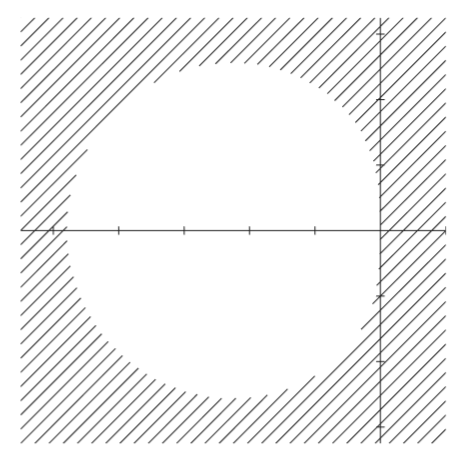
\includegraphics[width=0.7\textwidth]{lin-stab-a-m-2}%
		\caption{Область устйочивости двухшажного метода Адамса-Моултона}
		\vspace*{-2mm}
		\label{lin-stab-a-m-2}
	\end{figure}
	\end{columns}
	
\end{frame}	

\begin{frame}{Метод BDF}

\begin{block}{Расчетная формула для метода BDF-2}	
	\[
	y_{n+2} - \tfrac43 y_{n+1} + \tfrac13 y_n = \tfrac23 h f(t_{n+2}, y_{n+2})
	\]
\end{block}

\begin{block}{Расчетная формула для метода BDF-4}	
	\vspace{-3mm}
	\[
	y_{n+4} - \tfrac{48}{25} y_{n+3} + \tfrac{36}{25} y_{n+2} - \tfrac{16}{25} y_{n+1} + \tfrac{3}{25} y_n = \tfrac{12}{25} h f(t_{n+4}, y_{n+4})
	\]
\end{block}

%\vspace{-2mm}
\begin{columns}
	\column{0.5\textwidth}
	\begin{table}[!htbp]
		\centering
		\begin{tabular}{|l|l|l|} 
			\hline
			Шаг      & Разность     & Порядок            \\ 
			\hline
			0.1    & 2.57E-06 & 1.95  \\ 
			\hline
			0.05   & 7.36E-07 & 1.91  \\ 
			\hline
			0.025  & 1.96E-07 & 1.96  \\ 
			\hline
			0.0125 & 5.04E-08 &              \\
			\hline
		\end{tabular}
		\vspace*{4mm}
		\label{table-BDF-2}
		\caption{Порядки аппроксимации метода BDF-2}
	\end{table}
	
	\column{0.5\textwidth}
	\begin{table}[!htbp]
		\centering
		\begin{tabular}{|l|l|l|} 
			\hline
			Шаг      & Разность     & Порядок \\        \hline
			0.1    & 1.27E-10 & 3.94  \\ 
			\hline
			0.05   & 1.02E-11 & 3.99  \\ 
			\hline
			0.025  & 7.06E-13 & 3.93  \\ 
			\hline
			0.0125 & 4.64E-14 &              \\
			\hline
		\end{tabular}
		\vspace*{2mm}
		\label{table-BDF-4}
		\caption{Порядки аппроксимации метода BDF-4}
	\end{table}
\end{columns}

\end{frame}	

\begin{frame}{Области устойчивости методов BDF}
	
	\begin{columns}
		\column{0.5\textwidth}
		\begin{figure}[!htbp]
			\centering
			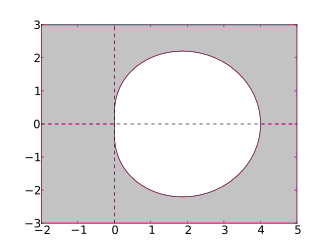
\includegraphics[width=1\textwidth]{330px-Stability_region_for_BDF2}%
			\caption{Область устойчивости метода BDF-2}
			\vspace*{-2mm}
			\label{ser_graph}
		\end{figure}
		\column{0.5\textwidth}
		\begin{figure}[!htbp]
			\centering
			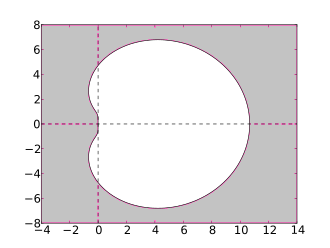
\includegraphics[width=1\textwidth]{330px-Stability_region_for_BDF4}%
			\caption{Область устойчивости метода BDF-4}
			\vspace*{-2mm}
			\label{ser_graph}
		\end{figure}
	\end{columns}

\end{frame}	

\begin{frame}{Фазовые траектории}
	
	\begin{columns}
	
	\column{0.4\textwidth}
	\begin{figure}[!htbp]
		\centering
		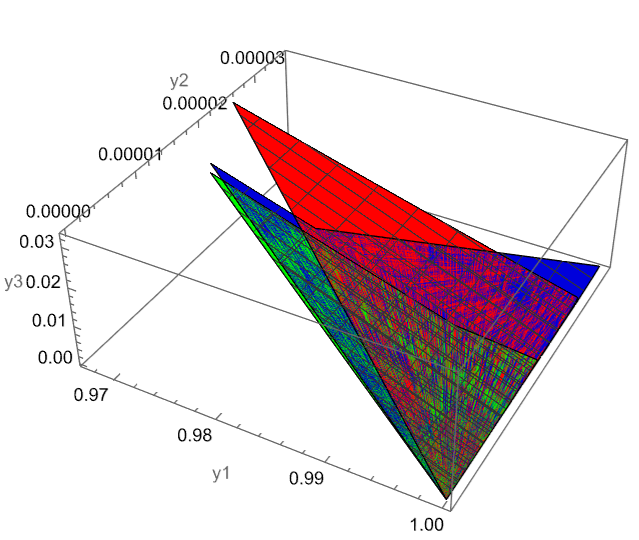
\includegraphics[width=0.7\textwidth]{T40-0}%
		\caption{Фазовые траектории при $T = 40$, $h = 10^-3$}
		\vspace*{-2mm}
		\label{T40-0}
	\end{figure}

	\column{0.4\textwidth}
	\begin{figure}[!htbp]
		\centering
		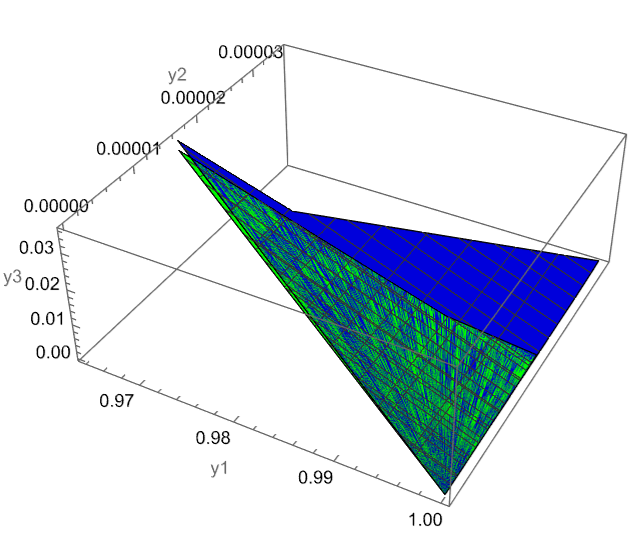
\includegraphics[width=0.7\textwidth]{T100-0}%
		\caption{Фазовые траектории при $T = 100$, $h = 10^-3$}
		\vspace*{-2mm}
		\label{T100-0}
	\end{figure}

	\column{0.4\textwidth}
	\begin{figure}[!htbp]
		\centering
		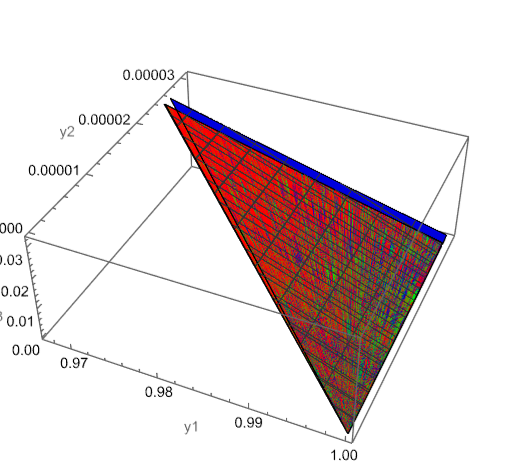
\includegraphics[width=0.7\textwidth]{T-40-s1000-0}%
		\caption{Фазовые траектории при $T = 40$, $h = 10^-4$}
		\vspace*{-2mm}
		\label{T-40-s1000-0}
	\end{figure}
	\end{columns}

	\begin{figure}[!htbp]
		\centering
		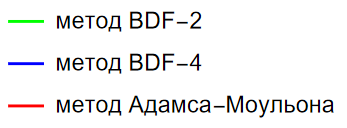
\includegraphics[width=0.4\textwidth]{graph-legend}%
	\end{figure}
\end{frame}

\begin{frame}{Графики зависимости $y_1$ от $t$}
	\begin{columns}
		
	\column{0.4\textwidth}
	\begin{figure}[!htbp]
		\centering
		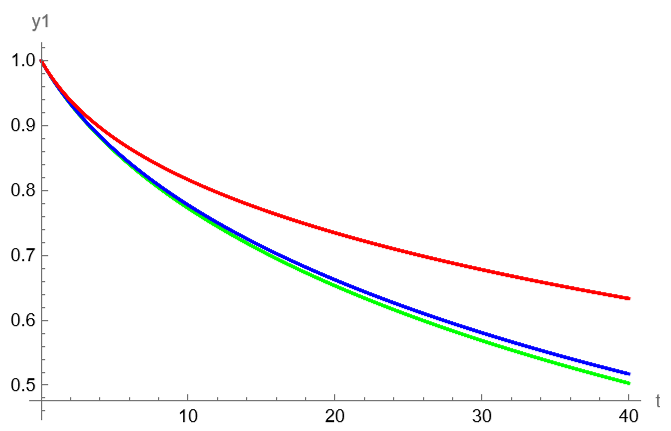
\includegraphics[width=0.9\textwidth]{T40-1}%
		\caption{Зависимость $y_1$ от $t$ при $T = 40$, $h = 10^-3$}
		\vspace*{-2mm}
		\label{T40-1}
	\end{figure}

	\column{0.4\textwidth}
	\begin{figure}[!htbp]
		\centering
		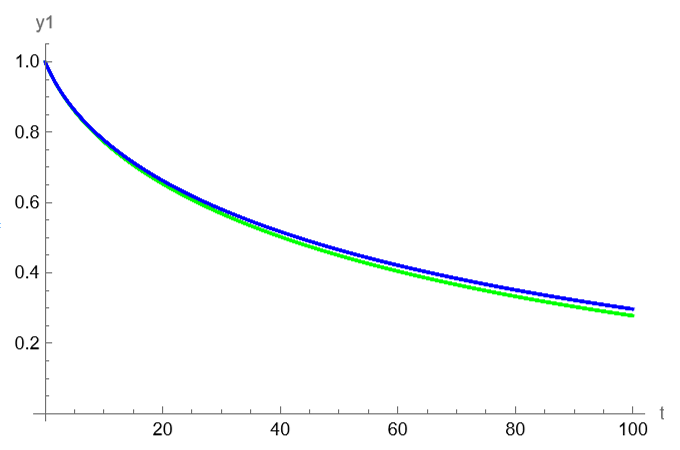
\includegraphics[width=0.9\textwidth]{T100-1}%
		\caption{Зависимость $y_1$ от $t$ при $T = 100$, $h = 10^-3$}
		\vspace*{-2mm}
		\label{T100-1}
	\end{figure}

	\column{0.4\textwidth}
	\begin{figure}[!htbp]
		\centering
		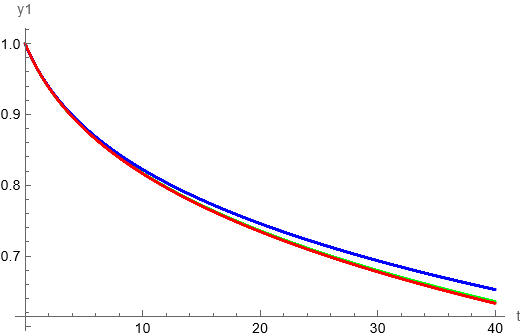
\includegraphics[width=0.9\textwidth]{T-40-s1000-1.png}%
		\caption{Зависимость $y_1$ от $t$ при $T = 40$, $h = 10^-4$}
		\vspace*{-2mm}
		\label{T-40-s1000-1.png}
	\end{figure}

	\end{columns}

	\begin{figure}[!htbp]
		\centering
		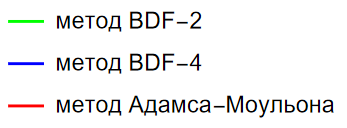
\includegraphics[width=0.4\textwidth]{graph-legend}%
	\end{figure}

\end{frame}

\begin{frame}{Графики зависимости $y_2$ от $t$}
	\begin{columns}
		
		\column{0.4\textwidth}
		\begin{figure}[!htbp]
			\centering
			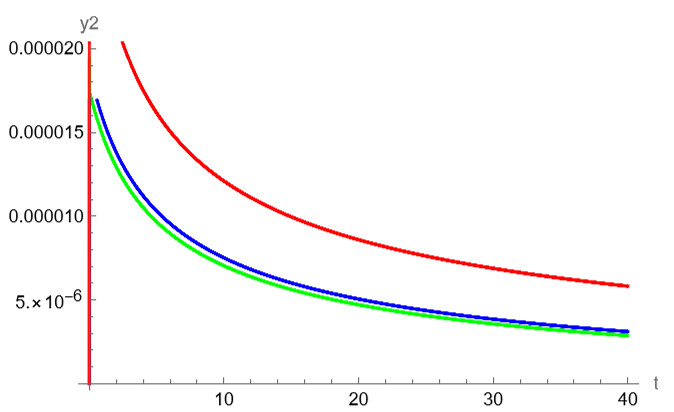
\includegraphics[width=0.9\textwidth]{T40-2}%
			\caption{Зависимость $y_2$ от $t$ при $T = 40$, $h = 10^-3$}
			\vspace*{-2mm}
			\label{T40-2}
		\end{figure}
		
		\column{0.4\textwidth}
		\begin{figure}[!htbp]
			\centering
			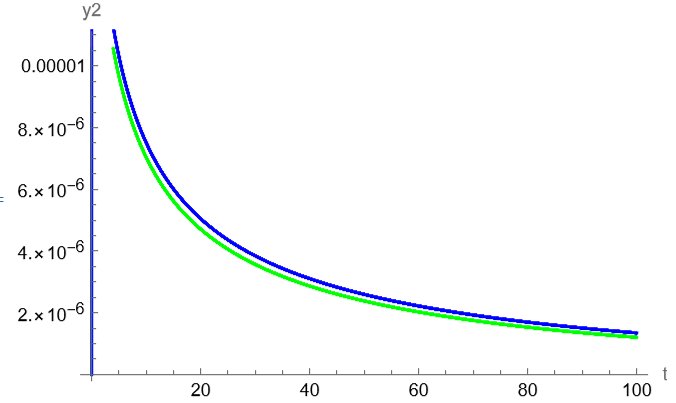
\includegraphics[width=0.9\textwidth]{T100-2}%
			\caption{Зависимость $y_2$ от $t$ при $T = 100$, $h = 10^-3$}
			\vspace*{-2mm}
			\label{T100-2}
		\end{figure}
	
	\column{0.4\textwidth}
	\begin{figure}[!htbp]
		\centering
		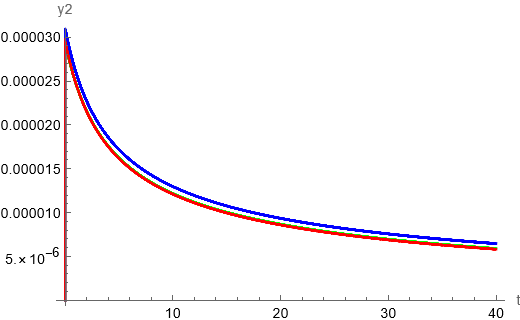
\includegraphics[width=0.9\textwidth]{T-40-s1000-2}%
		\caption{Зависимость $y_2$ от $t$ при $T = 40$, $h = 10^-4$}
		\vspace*{-2mm}
		\label{T-40-s1000-2}
	\end{figure}

	\end{columns}

	\begin{figure}[!htbp]
	\centering
	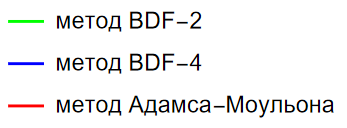
\includegraphics[width=0.4\textwidth]{graph-legend}
	\end{figure}
\end{frame}

\begin{frame}{Графики зависимости $y_3$ от $t$}
		\begin{columns}
		
		\column{0.4\textwidth}
		\begin{figure}[!htbp]
			\centering
			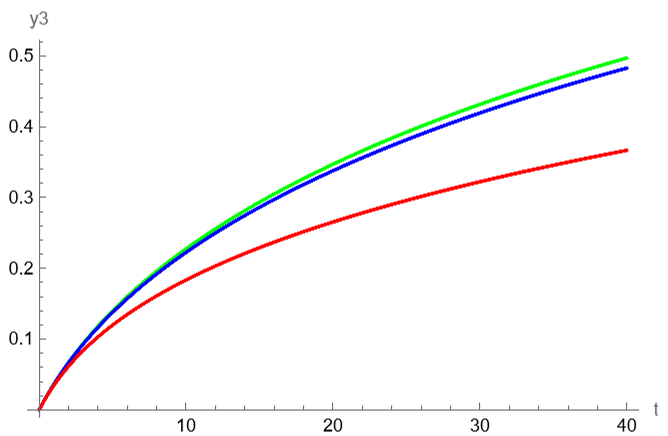
\includegraphics[width=0.9\textwidth]{T40-3}%
			\caption{Зависимость $y_3$ от $t$ при $T = 40$, $h = 10^-3$}
			\vspace*{-2mm}
			\label{T40-3}
		\end{figure}
			
		\column{0.4\textwidth}
		\begin{figure}[!htbp]
			\centering
			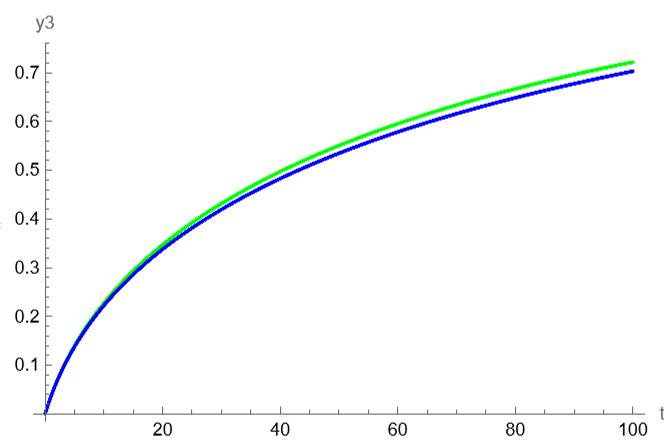
\includegraphics[width=0.9\textwidth]{T100-3}%
			\caption{Зависимость $y_3$ от $t$ при $T = 100$, $h = 10^-3$}
			\vspace*{-2mm}
			\label{T100-3}
		\end{figure}
	
		\column{0.4\textwidth}
		\begin{figure}[!htbp]
			\centering
			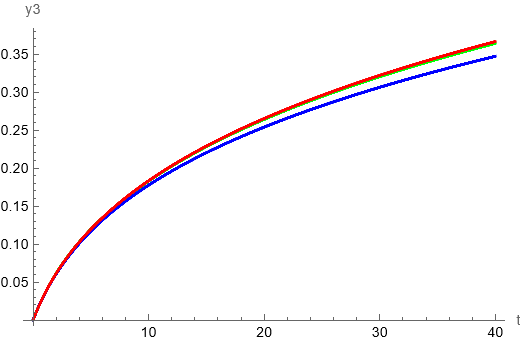
\includegraphics[width=0.9\textwidth]{T-40-s1000-3}%
			\caption{Зависимость $y_3$ от $t$ при $T = 40$, $h = 10^-4$}
			\vspace*{-2mm}
			\label{T-40-s1000-3}
		\end{figure}

	\end{columns}

	\begin{figure}[!htbp]
	\centering
	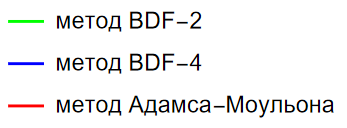
\includegraphics[width=0.4\textwidth]{graph-legend}
	\end{figure}
\end{frame}

\begin{frame}{Заключение}
	В ходе работы получены следующие результаты:
	\begin{block}{}
	\begin{enumerate}	
		\item Метод Адамса-Моултона является плохим выбором при решении жестких задач, так как он не является абсолютно устойчивым.
		\item В результатах расчетов решение для рассматриваемой задачи методом Адамса-Моултона удалось получить лишь на интервале $[0; 40]$.
		\item 
		Методы BDF-2 и BDF-4 позволили получить решение на поставленную задачу  как на интервале $[0; 40]$, так и на интервале $[0; 100]$.
	\end{enumerate}
	\end{block}	
\end{frame}	
\end{document} 